\section{Red Lentil Masala with Spinach}\index{vegetables!lentils!red lentil masala with spinach}

\begin{center}
Prep Time: 15 min
Cook Time: 30 min
Total Time: 45 min

\noindent Yield: 2 large (or 4 small) servings | Calories: 548 kcal

\vspace{1em}

  Source: Erin Alderson (https://naturallyella.com/red-lentils-and-spinach-in-masala-sauce/)
\end{center}

\subsection{Ingredients}
\subsubsection{Masala Paste}
\begin{multicols}{2}
\begin{itemize}
  \item 1 1/2   teaspoons cumin seeds
  \item 1 1/2   teaspoon coriander seeds
  \item 2   inch piece of ginger peeled and cut into pieces
  \item 1/8 to 3 teaspoons red pepper flakes see note
  \item 1   tablespoon smoked paprika
  \item 2   teaspoons garam marsala
  \item 1   teaspoon salt
  \item 2   tablespoons peanut oil or other nut oil
  \item 2   tablespoons tomato paste
  \item 1/3 cup packed cilantro leaves
\end{itemize}
\end{multicols}

\subsubsection{Lentils}
\begin{multicols}{2}
\begin{itemize}
  \item 1 tablespoon olive or coconut oil
  \item 1   small red onion diced
  \item 2   cloves garlic minced
  \item 1/3 cup masala paste
  \item 1   cup stewed tomatoes
  \item 1   cup coconut milk
  \item 1/2 cup red lentils
  \item 2   cups spinach packed
  \item 1/2 to 1 cup low-sodium vegetable broth
\end{itemize}
\end{multicols}

\subsection{Preparation}
\begin{enumerate}
  \item To make paste, toast cumin and coriander seeds in skillet until fragrant. Use a mortar and pestle (or a spice grinder) to grind spices.
  \item In a small food processor, add ginger and pulse until broken into small pieces. Add red pepper flakes, smoked paprika, cumin, coriander, garam marsala, and salt. Pulse a couple more times to incorporate. Next, add nut oil, tomato paste, and cilantro leaves. Pulse until paste forms and everything is well incorporated. Set aside.
  \item Heat a skillet over medium heat. Melt coconut oil and add diced onion, cooking until translucent, 4-5 minutes. Add in minced garlic and cook for one more minute.
  \item Stir in masala paste and cook for 1-2 minutes, then add stewed tomatoes and coconut milk. Stir together and bring to a boil.
  \item Add in lentils and reduce heat to low. Cook, stirring often, until lentils are tender, 20-25 minutes. If liquid has absorbed but lentils are still not tender, add 1/2 cup of vegetable broth and cook until lentils are tender. Remove from heat and fold in spinach.
  \item Serve with your favorite grain, extra cilantro, and a dollop of plain greek yogurt.
\end{enumerate}

\subsection{Recipe Notes}
\begin{description}
  \item [Tips and Tricks] I recommend making this dish once with the minimum amount of red pepper flakes in the masala paste and adding more crushed red pepper before serving if desired. The paste, with 3 teaspoons of red pepper flakes, can be really spicy.
  \item [Stock Up] Get the pantry ingredients you will need: coconut milk, stewed tomatoes, red lentils
  \item [Adapted From] http://www.marthastewart.com/319409/chicken-tikka-masala
\end{description}

\begin{figure}[h!]
    \centering
    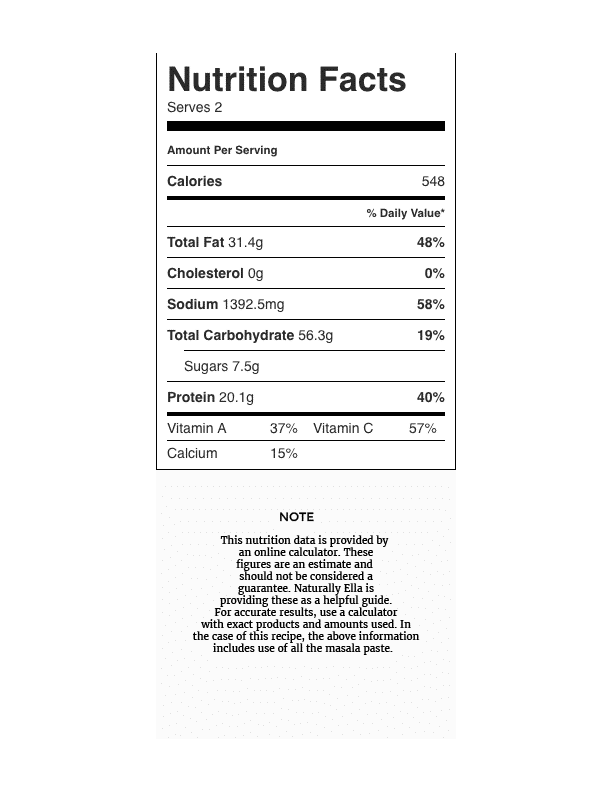
\includegraphics[width=.25\textwidth]{img/red-lentil-masala.png}
    \caption{Nutrition information for red lentil masala.}
    \label{fig:red-lentil-masala}
\end{figure}

